% Options for packages loaded elsewhere
\PassOptionsToPackage{unicode}{hyperref}
\PassOptionsToPackage{hyphens}{url}
\PassOptionsToPackage{dvipsnames,svgnames,x11names}{xcolor}
\documentclass[
  a4paper,
  11pt]{article}
\usepackage{xcolor}
\usepackage[margin=1in]{geometry}
\usepackage{amsmath,amssymb}
\setcounter{secnumdepth}{5}
\usepackage{iftex}
\ifPDFTeX
  \usepackage[T1]{fontenc}
  \usepackage[utf8]{inputenc}
  \usepackage{textcomp} % provide euro and other symbols
\else % if luatex or xetex
  \usepackage{unicode-math} % this also loads fontspec
  \defaultfontfeatures{Scale=MatchLowercase}
  \defaultfontfeatures[\rmfamily]{Ligatures=TeX,Scale=1}
\fi
\usepackage{lmodern}
\ifPDFTeX\else
  % xetex/luatex font selection
\fi
% Use upquote if available, for straight quotes in verbatim environments
\IfFileExists{upquote.sty}{\usepackage{upquote}}{}
\IfFileExists{microtype.sty}{% use microtype if available
  \usepackage[]{microtype}
  \UseMicrotypeSet[protrusion]{basicmath} % disable protrusion for tt fonts
}{}
\makeatletter
\@ifundefined{KOMAClassName}{% if non-KOMA class
  \IfFileExists{parskip.sty}{%
    \usepackage{parskip}
  }{% else
    \setlength{\parindent}{0pt}
    \setlength{\parskip}{6pt plus 2pt minus 1pt}}
}{% if KOMA class
  \KOMAoptions{parskip=half}}
\makeatother
\usepackage{color}
\usepackage{fancyvrb}
\newcommand{\VerbBar}{|}
\newcommand{\VERB}{\Verb[commandchars=\\\{\}]}
\DefineVerbatimEnvironment{Highlighting}{Verbatim}{commandchars=\\\{\}}
% Add ',fontsize=\small' for more characters per line
\newenvironment{Shaded}{}{}
\newcommand{\AlertTok}[1]{\textcolor[rgb]{1.00,0.00,0.00}{\textbf{#1}}}
\newcommand{\AnnotationTok}[1]{\textcolor[rgb]{0.38,0.63,0.69}{\textbf{\textit{#1}}}}
\newcommand{\AttributeTok}[1]{\textcolor[rgb]{0.49,0.56,0.16}{#1}}
\newcommand{\BaseNTok}[1]{\textcolor[rgb]{0.25,0.63,0.44}{#1}}
\newcommand{\BuiltInTok}[1]{\textcolor[rgb]{0.00,0.50,0.00}{#1}}
\newcommand{\CharTok}[1]{\textcolor[rgb]{0.25,0.44,0.63}{#1}}
\newcommand{\CommentTok}[1]{\textcolor[rgb]{0.38,0.63,0.69}{\textit{#1}}}
\newcommand{\CommentVarTok}[1]{\textcolor[rgb]{0.38,0.63,0.69}{\textbf{\textit{#1}}}}
\newcommand{\ConstantTok}[1]{\textcolor[rgb]{0.53,0.00,0.00}{#1}}
\newcommand{\ControlFlowTok}[1]{\textcolor[rgb]{0.00,0.44,0.13}{\textbf{#1}}}
\newcommand{\DataTypeTok}[1]{\textcolor[rgb]{0.56,0.13,0.00}{#1}}
\newcommand{\DecValTok}[1]{\textcolor[rgb]{0.25,0.63,0.44}{#1}}
\newcommand{\DocumentationTok}[1]{\textcolor[rgb]{0.73,0.13,0.13}{\textit{#1}}}
\newcommand{\ErrorTok}[1]{\textcolor[rgb]{1.00,0.00,0.00}{\textbf{#1}}}
\newcommand{\ExtensionTok}[1]{#1}
\newcommand{\FloatTok}[1]{\textcolor[rgb]{0.25,0.63,0.44}{#1}}
\newcommand{\FunctionTok}[1]{\textcolor[rgb]{0.02,0.16,0.49}{#1}}
\newcommand{\ImportTok}[1]{\textcolor[rgb]{0.00,0.50,0.00}{\textbf{#1}}}
\newcommand{\InformationTok}[1]{\textcolor[rgb]{0.38,0.63,0.69}{\textbf{\textit{#1}}}}
\newcommand{\KeywordTok}[1]{\textcolor[rgb]{0.00,0.44,0.13}{\textbf{#1}}}
\newcommand{\NormalTok}[1]{#1}
\newcommand{\OperatorTok}[1]{\textcolor[rgb]{0.40,0.40,0.40}{#1}}
\newcommand{\OtherTok}[1]{\textcolor[rgb]{0.00,0.44,0.13}{#1}}
\newcommand{\PreprocessorTok}[1]{\textcolor[rgb]{0.74,0.48,0.00}{#1}}
\newcommand{\RegionMarkerTok}[1]{#1}
\newcommand{\SpecialCharTok}[1]{\textcolor[rgb]{0.25,0.44,0.63}{#1}}
\newcommand{\SpecialStringTok}[1]{\textcolor[rgb]{0.73,0.40,0.53}{#1}}
\newcommand{\StringTok}[1]{\textcolor[rgb]{0.25,0.44,0.63}{#1}}
\newcommand{\VariableTok}[1]{\textcolor[rgb]{0.10,0.09,0.49}{#1}}
\newcommand{\VerbatimStringTok}[1]{\textcolor[rgb]{0.25,0.44,0.63}{#1}}
\newcommand{\WarningTok}[1]{\textcolor[rgb]{0.38,0.63,0.69}{\textbf{\textit{#1}}}}
\usepackage{longtable,booktabs,array}
\newcounter{none} % for unnumbered tables
\usepackage{calc} % for calculating minipage widths
% Correct order of tables after \paragraph or \subparagraph
\usepackage{etoolbox}
\makeatletter
\patchcmd\longtable{\par}{\if@noskipsec\mbox{}\fi\par}{}{}
\makeatother
% Allow footnotes in longtable head/foot
\IfFileExists{footnotehyper.sty}{\usepackage{footnotehyper}}{\usepackage{footnote}}
\makesavenoteenv{longtable}
\usepackage{graphicx}
\makeatletter
\newsavebox\pandoc@box
\newcommand*\pandocbounded[1]{% scales image to fit in text height/width
  \sbox\pandoc@box{#1}%
  \Gscale@div\@tempa{\textheight}{\dimexpr\ht\pandoc@box+\dp\pandoc@box\relax}%
  \Gscale@div\@tempb{\linewidth}{\wd\pandoc@box}%
  \ifdim\@tempb\p@<\@tempa\p@\let\@tempa\@tempb\fi% select the smaller of both
  \ifdim\@tempa\p@<\p@\scalebox{\@tempa}{\usebox\pandoc@box}%
  \else\usebox{\pandoc@box}%
  \fi%
}
% Set default figure placement to htbp
\def\fps@figure{htbp}
\makeatother
\setlength{\emergencystretch}{3em} % prevent overfull lines
\providecommand{\tightlist}{%
  \setlength{\itemsep}{0pt}\setlength{\parskip}{0pt}}
\usepackage{bookmark}
\IfFileExists{xurl.sty}{\usepackage{xurl}}{} % add URL line breaks if available
\urlstyle{same}
\hypersetup{
  colorlinks=true,
  linkcolor={blue},
  filecolor={Maroon},
  citecolor={Blue},
  urlcolor={blue},
  pdfcreator={LaTeX via pandoc}}

\author{}
\date{}

\begin{document}

{
\setcounter{tocdepth}{3}
\tableofcontents
}
\section{Insider Threat Detection on CMU-CERT r4.2: A Comparative Study
of Behavioral Sequence Matching and Heterogeneous Graph Neural
Networks}\label{insider-threat-detection-on-cmu-cert-r42-a-comparative-study-of-behavioral-sequence-matching-and-heterogeneous-graph-neural-networks}

Report Date: 2026-05-26

\begin{center}\rule{0.5\linewidth}{0.5pt}\end{center}

\subsection{Abstract}\label{abstract}

Insider threat detection faces fundamental challenges including label
scarcity, long behavioral time spans, stealthy attack chains, and high
false-positive costs. This project uses the CMU-CERT r4.2 dataset
(\textasciitilde16 GB / 1,000 employees / 17 months of logs / 70
malicious users) to implement and compare two insider threat detection
approaches:

\begin{itemize}
\tightlist
\item
  \textbf{Approach 1: N-gram Template-Based Behavioral Sequence
  Matching} --- abstracts multi-source logs into unified behavioral
  token time series and generates user-level risk scores through a
  weighted fusion of four complementary detectors (red-team template
  matching, N-gram language model anomaly, malicious signature
  similarity, and peer rarity deviation);
\item
  \textbf{Approach 2: R-GCN Heterogeneous Graph Detection} ---
  constructs a heterogeneous graph over users, PCs, file types, and URL
  categories, then applies Relational Graph Convolutional Networks
  (R-GCN) for semi-supervised node classification, automatically
  learning structural features that distinguish malicious from benign
  users.
\end{itemize}

Comparative experiments on the full r4.2 dataset demonstrate that R-GCN
comprehensively outperforms the N-gram approach across all core metrics:
ROC-AUC reaches \textbf{0.9898} (vs. 0.9041 for N-gram), PR-AUC reaches
\textbf{0.8358} (vs. 0.3257), and Top-100 Recall reaches
\textbf{98.57\%} (vs. 52.86\%). R-GCN shows particularly striking
improvement on the hardest-to-detect S2 scenario (job-hunting + email
exfiltration), where Top-100 Recall jumps from 16.67\% to 96.67\%.
However, the N-gram approach retains unique advantages in
interpretability, as each high-risk user can be traced back to specific
rule templates and behavioral patterns.

\subsection{1. Background and
Motivation}\label{1-background-and-motivation}

Enterprise insider threats typically do not manifest as single isolated
events, but rather as a set of temporally correlated behaviors --- such
as after-hours logins, removable storage device connections, visits to
leak sites, copying sensitive files, or sending attachments to external
email addresses. Single-point anomaly detection is easily disrupted by
office noise, while purely supervised learning requires large amounts of
high-quality labels that are difficult to obtain in real-world
environments.

CMU-CERT r4.2 is a widely used simulated dataset in insider threat
detection research, containing multi-month, multi-source logs with
red-team-injected malicious user behaviors. This dataset is well-suited
for studying the following questions:

\begin{itemize}
\tightlist
\item
  How to convert heterogeneous logs into unified user behavioral
  sequences;
\item
  How to extract ordered behavioral patterns from attack playbooks;
\item
  How to establish anomaly baselines using benign population behavior
  under label-scarce conditions;
\item
  How to leverage graph-structural relationships among users, devices,
  and resources to enhance detection;
\item
  How to preserve interpretability in detection results to assist
  security analysts in investigation.
\end{itemize}

This project pursues two technical approaches: a domain-knowledge-driven
"behavioral sequence matching" method and a data-driven "heterogeneous
graph neural network" method, conducting a rigorous comparison on the
same dataset to inform practical deployment decisions.

\subsection{2. Dataset and Threat
Scenarios}\label{2-dataset-and-threat-scenarios}

\subsubsection{2.1 Dataset Overview}\label{21-dataset-overview}

The project is based on the CMU-CERT r4.2 dataset. The raw data is
approximately 16 GB, covering 1,000 employees over approximately 17
months of enterprise activity logs:

{\def\LTcaptype{none} % do not increment counter
\begin{longtable}[]{@{}lrll@{}}
\toprule\noalign{}
Data Source & File Size & Key Fields & Behavioral Meaning \\
\midrule\noalign{}
\endhead
\bottomrule\noalign{}
\endlastfoot
logon.csv & 56 MB & date, user, pc, activity & Login/logout events;
identifies work hours, after-hours, and whether the
user\textquotesingle s own PC is used \\
device.csv & 28 MB & date, user, pc, activity & USB device
connect/disconnect events \\
file.csv & 184 MB & date, user, pc, filename & File access events,
classified by document, executable, and other types \\
http.csv & 14.5 GB & date, user, pc, url, content & HTTP browsing
events; project generates a slim version http\_slim.csv (4.1 GB) \\
email.csv & 1.3 GB & date, user, recipients, attachments &
Internal/external email and attachment exfiltration events \\
LDAP/ & \textasciitilde2.5 MB & user, role, department, team & Employee
position and organizational attributes (monthly snapshots) \\
insiders.csv & 14 KB & dataset, scenario, user, start, end & Official
malicious user ground truth \\
\end{longtable}
}

\subsubsection{2.2 Threat Scenario
Definitions}\label{22-threat-scenario-definitions}

The project uses the r4.2 malicious user list verified against the
official \texttt{insiders.csv} in \texttt{src/build\_ground\_truth.py},
totaling \textbf{70 unique malicious users} across three typical
scenarios:

{\def\LTcaptype{none} % do not increment counter
\begin{longtable}[]{@{}lrl@{}}
\toprule\noalign{}
Scenario & Users & Attack Playbook \\
\midrule\noalign{}
\endhead
\bottomrule\noalign{}
\endlastfoot
S1: Data Leak / USB Exfiltration & 30 & Disgruntled or departing
employees log in after hours, connect USB drives, access or copy
documents, and upload to leak sites (wikileaks) \\
S2: Pre-Departure Data Exfiltration & 30 & Employees browse job-hunting
websites, steal competitive or business materials, and exfiltrate via
personal email or external email channels \\
S3: Sysadmin Keylogger & 10 & Administrators visit keylogger sites,
install executables, and send destructive emails impersonating
executives \\
\end{longtable}
}

The three scenarios are mutually exclusive, covering 70 malicious users
and 930 benign users in total.

\subsection{3. Data Preprocessing and Behavioral
Tokenization}\label{3-data-preprocessing-and-behavioral-tokenization}

\subsubsection{3.1 Unified Preprocessing
Pipeline}\label{31-unified-preprocessing-pipeline}

The preprocessing script is \texttt{src/preprocess.py}. Its core idea is
to stream-read multi-source logs and unify them into per-user,
chronologically-ordered behavioral token sequences.

\textbf{Temporal Context Segmentation}:

\begin{itemize}
\tightlist
\item
  Work Hours (WH): Monday through Friday, 07:00--18:00;
\item
  After Hours (AH): weekends, late nights, early mornings, and all other
  non-work periods.
\end{itemize}

\textbf{User Context Identification}:

\begin{itemize}
\tightlist
\item
  The most frequently used PC for each user is identified from logon
  logs as their "primary PC";
\item
  Login events are differentiated into \texttt{LOGON\_WH\_OWN}
  (work-hours login on own PC), \texttt{LOGON\_AH\_OTHER} (after-hours
  login on another\textquotesingle s PC), etc.
\end{itemize}

\subsubsection{3.2 Behavioral Token
Vocabulary}\label{32-behavioral-token-vocabulary}

The project defines approximately 30 behavioral token types.
Representative examples:

{\def\LTcaptype{none} % do not increment counter
\begin{longtable}[]{@{}lll@{}}
\toprule\noalign{}
Category & Token Example & Meaning \\
\midrule\noalign{}
\endhead
\bottomrule\noalign{}
\endlastfoot
Logon & \texttt{LOGON\_AH\_OTHER} & After-hours login on a non-primary
PC \\
Device & \texttt{USB\_CONN\_AH} & After-hours USB device connection \\
File & \texttt{FILE\_DOC\_AH} & After-hours document file access \\
File & \texttt{FILE\_EXEC\_WH} & Work-hours executable file access \\
HTTP & \texttt{HTTP\_LEAK\_AH} & After-hours visit to a leak-related
site \\
HTTP & \texttt{HTTP\_KEYLOG\_WH} & Work-hours visit to a
keylogger-related site \\
HTTP & \texttt{HTTP\_JOBHUNT\_WH} & Work-hours visit to a job-hunting
site \\
Email & \texttt{EMAIL\_EXT\_ATT\_WH} & Work-hours email with attachment
to external recipient \\
\end{longtable}
}

Complete preprocessing output: \textbf{1,000 users, 4,779,378 events},
saved as \texttt{outputs/user\_sequences.pkl} and
\texttt{outputs/user\_daily\_seq.pkl}.

\subsubsection{3.3 HTTP Data Slimming}\label{33-http-data-slimming}

The raw \texttt{http.csv} file is 14.5 GB, primarily due to the bulky
\texttt{content} field. The project generates a slim version via
\texttt{src/generate\_http\_slim.py} --- \texttt{http\_slim.csv} (4.1
GB, 28,434,423 rows) --- retaining only the five columns
\texttt{id,\ date,\ user,\ pc,\ url} for use by both algorithms.

\subsection{4. Approach 1: N-gram Template-Based Behavioral Sequence
Matching}\label{4-approach-1-n-gram-template-based-behavioral-sequence-matching}

\subsubsection{4.1 Method Overview}\label{41-method-overview}

This approach is defined in \texttt{src/sequence\_matching.py}. The
overall architecture is:

\begin{Shaded}
\begin{Highlighting}[]
\NormalTok{Multi{-}source Logs}
\NormalTok{  {-}\textgreater{} Behavioral Token Sequence}
\NormalTok{  {-}\textgreater{} PatternRule / NGramAnomaly / SequenceSimilarity / PeerDeviation}
\NormalTok{  {-}\textgreater{} Component Normalization}
\NormalTok{  {-}\textgreater{} User Risk Score R(u)}
\NormalTok{  {-}\textgreater{} Ranking, Top{-}K Metrics, and Explanations}
\end{Highlighting}
\end{Shaded}

The system consists of four complementary detectors, all following a
"higher score = more suspicious" convention. Outputs are min-max
normalized and linearly fused into a final risk score.

\subsubsection{4.2 Threat Weight Design}\label{42-threat-weight-design}

Based on the prevalence ratio of each token between malicious and benign
users, the project assigns data-driven threat weights (approximating
\texttt{log(P(t\textbar{}malicious)\ /\ P(t\textbar{}benign))}):

{\def\LTcaptype{none} % do not increment counter
\begin{longtable}[]{@{}lrrl@{}}
\toprule\noalign{}
Token & Weight & Mal/Ben Ratio & Interpretation \\
\midrule\noalign{}
\endhead
\bottomrule\noalign{}
\endlastfoot
\texttt{HTTP\_LEAK\_AH/WH} & 8.0 & 39--52× & Visiting leak sites; very
strong malicious signal \\
\texttt{HTTP\_KEYLOG\_AH/WH} & 8.0 & 38× & Visiting keylogger sites;
very strong malicious signal \\
\texttt{USB\_CONN\_AH} & 2.5 & 5.3× & After-hours removable device
connection \\
\texttt{FILE\_EXEC\_AH} & 2.0 & 3.5× & After-hours executable file
access \\
\texttt{LOGON\_AH\_OTHER} & 2.0 & 1.7× & After-hours login on a
non-primary PC \\
\texttt{HTTP\_JOBHUNT\_WH} & 0.0 & 1.1× & Job-hunting sites appear in
83\% of benign users; extremely low discriminative power \\
\end{longtable}
}

\subsubsection{4.3 The Four Detectors}\label{43-the-four-detectors}

\textbf{(1) PatternRule: Red-Team Playbook Ordered Subsequence Matching}

Encodes three red-team scenarios into 21 behavioral templates. For
example, S1 includes combinations such as
\texttt{{[}LOGON\_AH\_OWN,\ USB\_CONN\_AH,\ FILE\_DOC\_AH{]}}. Performs
ordered subsequence matching within a sliding window (default size 15)
with non-overlapping counting:

\begin{Shaded}
\begin{Highlighting}[]
\NormalTok{score(pattern) = log(1 + hits) × len(pattern)\^{}1.5 × (1 + Σ threat\_weight(token))}
\end{Highlighting}
\end{Shaded}

\textbf{(2) NGramAnomaly: Benign Behavior Language Model}

Trains a 3-gram language model (additive smoothing α=0.5) on 70\% of
benign users and computes the perplexity of each test
user\textquotesingle s sequence. Higher perplexity indicates greater
deviation from normal behavioral patterns.

\textbf{(3) SequenceSimilarity: Malicious Signature Similarity}

Concatenates each scenario\textquotesingle s template tokens into
malicious signature sequences and computes the Longest Common
Subsequence (LCS) ratio between the user\textquotesingle s behavioral
sequence and the signatures, with weighted counting of high-sensitivity
token occurrences:

\begin{Shaded}
\begin{Highlighting}[]
\NormalTok{score = 0.4 × LCS\_ratio + 0.6 × weighted\_high\_sensitive\_hit}
\end{Highlighting}
\end{Shaded}

\textbf{(4) PeerDeviation: High-Risk Token Peer Rarity}

Focuses exclusively on the 9 token types with threat weight ≥ 1.5,
computing IDF-weighted deviation scores:

\begin{Shaded}
\begin{Highlighting}[]
\NormalTok{score = Σ log(1 + count\_u(token)) × IDF(token) × threat\_weight(token)}
\end{Highlighting}
\end{Shaded}

\subsubsection{4.4 Fusion Strategy}\label{44-fusion-strategy}

The four detector outputs undergo min-max normalization followed by
linear fusion:

\begin{Shaded}
\begin{Highlighting}[]
\NormalTok{R(u) = 0.40 × z(rule) + 0.20 × z(perplexity) + 0.25 × z(similarity) + 0.15 × z(peer)}
\end{Highlighting}
\end{Shaded}

Weights are manually specified, emphasizing rule matching and similarity
signals.

\subsection{5. Approach 2: R-GCN Heterogeneous Graph
Detection}\label{5-approach-2-r-gcn-heterogeneous-graph-detection}

\subsubsection{5.1 Method Overview}\label{51-method-overview}

This approach formulates insider threat detection as a node
classification problem on a heterogeneous graph, using Relational Graph
Convolutional Networks (R-GCN) to automatically learn user-level
malicious features from graph structure. The code resides in
\texttt{src/rgcn/}.

\subsubsection{5.2 Heterogeneous Graph
Construction}\label{52-heterogeneous-graph-construction}

The graph construction script is \texttt{src/rgcn/build\_graph.py},
which builds a heterogeneous graph from the full r4.2 data containing 4
node types and 6 relation types:

\textbf{Node Types (4 types, 2,017 total nodes)}:

{\def\LTcaptype{none} % do not increment counter
\begin{longtable}[]{@{}lrl@{}}
\toprule\noalign{}
Node Type & Count & Description \\
\midrule\noalign{}
\endhead
\bottomrule\noalign{}
\endlastfoot
user & 1,000 & Employee nodes \\
pc & 1,003 & Workstation nodes \\
file\_type & 6 & File category nodes: (doc/exec/other) × (WH/AH) \\
url\_cat & 8 & URL category nodes: (LEAK/KEYLOG/JOBHUNT/OTHER) ×
(WH/AH) \\
\end{longtable}
}

\textbf{Relation Types (6 types, 38,568 total edges)}:

{\def\LTcaptype{none} % do not increment counter
\begin{longtable}[]{@{}llrl@{}}
\toprule\noalign{}
Relation & Direction & Edges & Meaning \\
\midrule\noalign{}
\endhead
\bottomrule\noalign{}
\endlastfoot
logon\_wh & user → pc & 8,074 & Work-hours logins \\
logon\_ah & user → pc & 20,144 & After-hours logins \\
usb\_wh & user → pc & 1,441 & Work-hours USB connections \\
usb\_ah & user → pc & 4,639 & After-hours USB connections \\
file\_op & user → file\_type & 1,063 & File operations \\
http\_visit & user → url\_cat & 3,207 & HTTP browsing \\
\end{longtable}
}

Each edge carries a weight \texttt{w\ =\ log(1\ +\ count)}, and multiple
occurrences of the same \texttt{(src,\ dst,\ rel)} are merged. Reverse
edges are automatically added during training, giving the R-GCN 12
relation types in total.

\textbf{User Node Features (6-dimensional)}:

\begin{enumerate}
\def\labelenumi{\arabic{enumi}.}
\tightlist
\item
  Number of active days
\item
  Total event count
\item
  After-hours event ratio
\item
  Number of distinct PCs used
\item
  Number of distinct file types accessed
\item
  After-hours login count
\end{enumerate}

Features are standardized using RobustScaler (subtract median / divide
by IQR) and clipped to {[}-5, 5{]}.

\subsubsection{5.3 R-GCN Model
Architecture}\label{53-r-gcn-model-architecture}

The model is implemented in \texttt{src/rgcn/rgcn\_model.py}, following
the R-GCN framework of Schlichtkrull et al. (ESWC 2018) in pure PyTorch
(no DGL/PyG dependency).

\textbf{Core Formula}:

\begin{Shaded}
\begin{Highlighting}[]
\NormalTok{h\_v\^{}(l+1) = σ( W\_self × h\_v\^{}(l) + Σ\_r Σ\_\{u∈N\_r(v)\} (w\_\{u,v,r\} / c\_\{v,r\}) × W\_r × h\_u\^{}(l) )}
\end{Highlighting}
\end{Shaded}

where \texttt{W\_r} employs basis decomposition:
\texttt{W\_r\ =\ Σ\_\{b=1..B\}\ a\_\{rb\}\ ×\ V\_b}, sharing B=4 basis
matrices across 12 relations to effectively reduce parameter count.

\textbf{Model Structure}:

\begin{Shaded}
\begin{Highlighting}[]
\NormalTok{user: Linear(6, 64)  ─┐}
\NormalTok{pc:   Embedding(64)   ─┤}
\NormalTok{file: Embedding(64)   ─┼──→ R{-}GCN Layer 1 (64→64, ReLU) ──→ R{-}GCN Layer 2 (64→64)}
\NormalTok{url:  Embedding(64)   ─┘                                          │}
\NormalTok{                                                                   ↓}
\NormalTok{                                                    Linear(64→32) → ReLU → Linear(32→1)}
\NormalTok{                                                    (user nodes only)    → sigmoid → P(malicious)}
\end{Highlighting}
\end{Shaded}

\subsubsection{5.4 Training Strategy}\label{54-training-strategy}

\begin{itemize}
\tightlist
\item
  \textbf{Semi-supervised Transductive}: all nodes participate in
  message passing, but loss is computed only on training nodes;
\item
  \textbf{5-fold StratifiedKFold} cross-validation, preserving
  malicious/benign ratio in each fold;
\item
  \textbf{Class Imbalance Handling}: BCEWithLogitsLoss with
  \texttt{pos\_weight\ =\ \#neg\ /\ \#pos\ ≈\ 13.3};
\item
  \textbf{Optimizer}: AdamW, lr=0.01, weight\_decay=5e-4;
\item
  \textbf{Early Stopping}: patience=50 epochs, monitoring validation
  ROC-AUC;
\item
  \textbf{Gradient Clipping}: max\_norm=2.0;
\item
  \textbf{Out-of-Fold (OOF) Prediction}: each user receives a score from
  the fold where it served as validation, then all scores are aggregated
  for overall metrics.
\end{itemize}

\subsubsection{5.5 Hyperparameter
Configuration}\label{55-hyperparameter-configuration}

{\def\LTcaptype{none} % do not increment counter
\begin{longtable}[]{@{}lll@{}}
\toprule\noalign{}
Parameter & Value & Description \\
\midrule\noalign{}
\endhead
\bottomrule\noalign{}
\endlastfoot
hidden\_dim & 64 & Hidden layer dimension \\
num\_layers & 2 & Number of R-GCN layers \\
num\_bases & 4 & Basis decomposition rank \\
dropout & 0.3 & Dropout rate \\
lr & 0.01 & Learning rate \\
weight\_decay & 5e-4 & Weight decay \\
epochs & 300 & Maximum training epochs \\
patience & 50 & Early stopping patience \\
n\_splits & 5 & Cross-validation folds \\
\end{longtable}
}

\subsection{6. Experimental Design}\label{6-experimental-design}

\subsubsection{6.1 Evaluation Framework}\label{61-evaluation-framework}

Both algorithms are evaluated on the identical dataset:

{\def\LTcaptype{none} % do not increment counter
\begin{longtable}[]{@{}lll@{}}
\toprule\noalign{}
Item & N-gram Approach & R-GCN Approach \\
\midrule\noalign{}
\endhead
\bottomrule\noalign{}
\endlastfoot
Dataset & Full r4.2 (1,000 users) & Full r4.2 (1,000 users) \\
Data Sources & logon + device + file + http\_slim + email & logon +
device + file + http\_slim \\
Evaluation Protocol & 70\% benign train / 30\% held-out + full scoring &
5-fold StratifiedKFold + OOF aggregation \\
Label Usage & Evaluation only (unsupervised scoring) & Training binary
classifier (semi-supervised) \\
Ground Truth & 70 malicious users (S1:30, S2:30, S3:10) & 70 malicious
users (S1:30, S2:30, S3:10) \\
\end{longtable}
}

\subsubsection{6.2 Evaluation Metrics}\label{62-evaluation-metrics}

\begin{itemize}
\tightlist
\item
  \textbf{ROC-AUC}: True positive rate vs. false positive rate trade-off
  across thresholds;
\item
  \textbf{PR-AUC}: Particularly informative under sparse positive
  samples (7\%), reflecting practical investigation difficulty;
\item
  \textbf{Top-K Precision/Recall} (K=10, 20, 30, 50, 70, 100): Simulates
  the "prioritize reviewing the top K users" scenario in security
  operations;
\item
  \textbf{Scenario-Level Recall}: Per-scenario (S1/S2/S3) recall within
  Top-70 and Top-100.
\end{itemize}

\subsection{7. Experimental Results}\label{7-experimental-results}

\subsubsection{7.1 Overall Performance
Comparison}\label{71-overall-performance-comparison}

{\def\LTcaptype{none} % do not increment counter
\begin{longtable}[]{@{}lrrr@{}}
\toprule\noalign{}
Metric & N-gram & R-GCN & R-GCN Improvement \\
\midrule\noalign{}
\endhead
\bottomrule\noalign{}
\endlastfoot
\textbf{ROC-AUC} & 0.9041 & \textbf{0.9898} & +9.5\% \\
\textbf{PR-AUC} & 0.3257 & \textbf{0.8358} & +156.6\% \\
\end{longtable}
}

R-GCN leads comprehensively across both core metrics. The PR-AUC gap is
especially notable (0.33 vs. 0.84), indicating that R-GCN maintains high
precision even at elevated recall levels, whereas the N-gram approach
suffers rapid precision degradation when pursuing high recall.

The R-GCN 5-fold cross-validation results are also highly stable:
per-fold AUCs are {[}0.9981, 0.9923, 0.9939, 0.9866, 0.9885{]}, mean
\textbf{0.9919 ± 0.0041}.

\pandocbounded{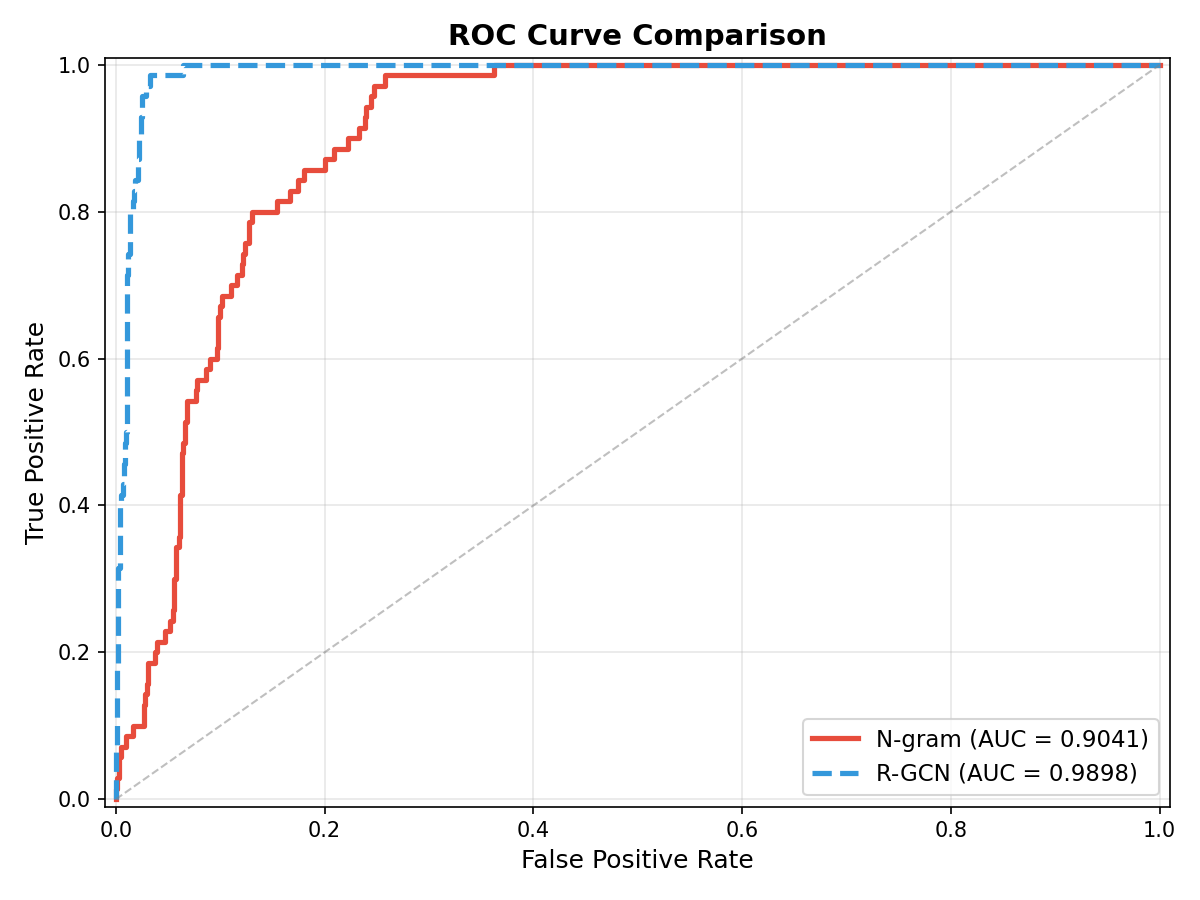
\includegraphics[keepaspectratio,alt={ROC Curve Comparison}]{outputs/comparison/fig_roc_comparison.png}}

Figure 1 shows the ROC curves of the two approaches. The R-GCN curve
stays closer to the upper-left corner, indicating a consistently higher
true positive rate and lower false positive rate across thresholds.

\pandocbounded{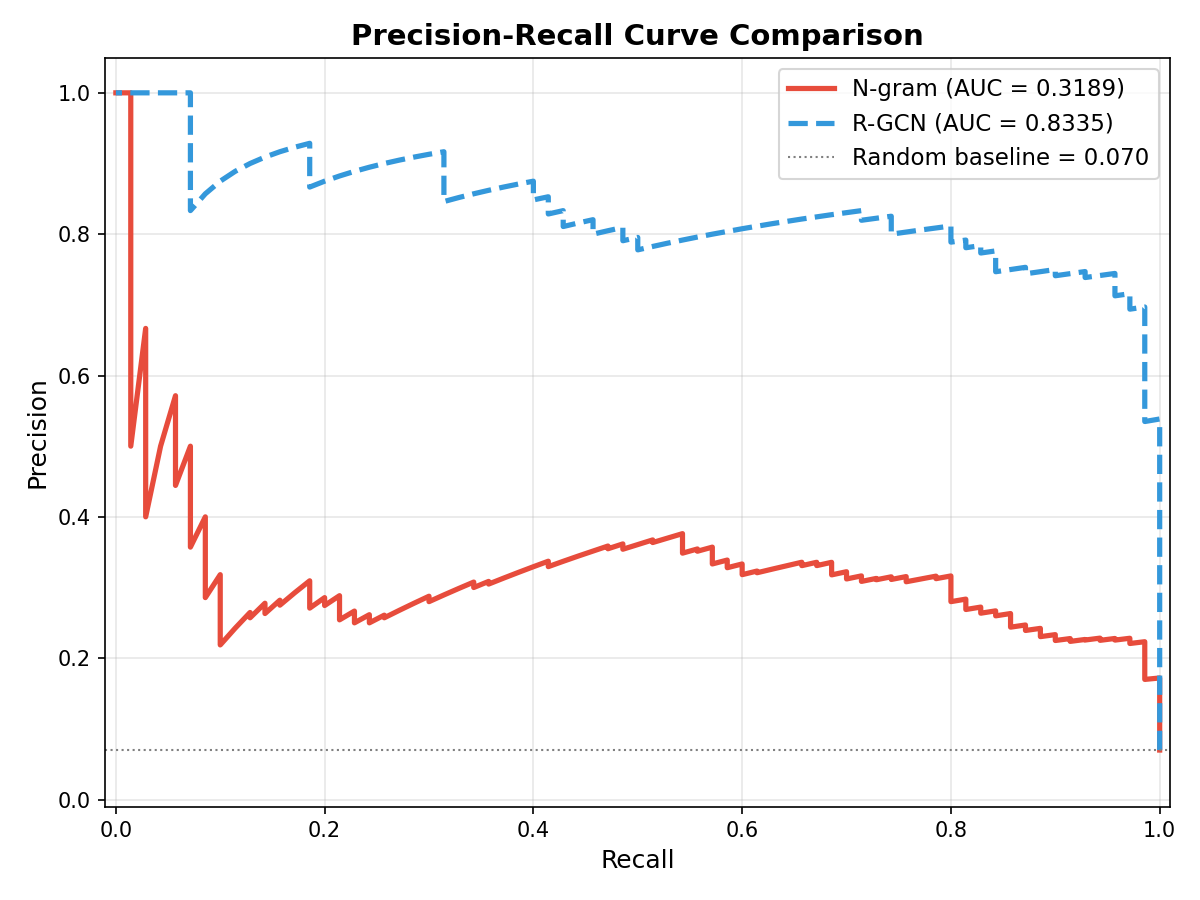
\includegraphics[keepaspectratio,alt={Precision-Recall Curve Comparison}]{outputs/comparison/fig_pr_comparison.png}}

Figure 2 shows the Precision-Recall curves. Since malicious users
account for only 7\% of all users, PR curves better reflect the
practical investigation burden; R-GCN remains substantially above
N-gram, especially in high-recall regions.

\subsubsection{7.2 Top-K Investigation Effectiveness
Comparison}\label{72-top-k-investigation-effectiveness-comparison}

In security operations, analysts typically prioritize the highest-ranked
users, making Top-K metrics more practically relevant than
classification thresholds.

{\def\LTcaptype{none} % do not increment counter
\begin{longtable}[]{@{}rrrrrrr@{}}
\toprule\noalign{}
K & N-gram Prec & R-GCN Prec & N-gram Rec & R-GCN Rec & N-gram Hits &
R-GCN Hits \\
\midrule\noalign{}
\endhead
\bottomrule\noalign{}
\endlastfoot
10 & 0.50 & \textbf{0.90} & 0.07 & \textbf{0.13} & 5 & 9 \\
20 & 0.30 & \textbf{0.90} & 0.09 & \textbf{0.26} & 6 & 18 \\
30 & 0.23 & \textbf{0.87} & 0.10 & \textbf{0.37} & 7 & 26 \\
50 & 0.28 & \textbf{0.80} & 0.20 & \textbf{0.57} & 14 & 40 \\
70 & 0.26 & \textbf{0.80} & 0.26 & \textbf{0.80} & 18 & 56 \\
100 & 0.37 & \textbf{0.69} & 0.53 & \textbf{0.99} & 37 & 69 \\
\end{longtable}
}

Key findings:

\begin{itemize}
\tightlist
\item
  R-GCN identifies 9/70 malicious users in the Top-10 (90\% precision);
  N-gram identifies only 5 (50\% precision);
\item
  R-GCN achieves 80\% recall at Top-70 (56/70), while N-gram achieves
  only 53\% at Top-100 (37/70);
\item
  R-GCN identifies 69/70 malicious users in the Top-100 (missing only
  1), approaching perfect recall.
\end{itemize}

\pandocbounded{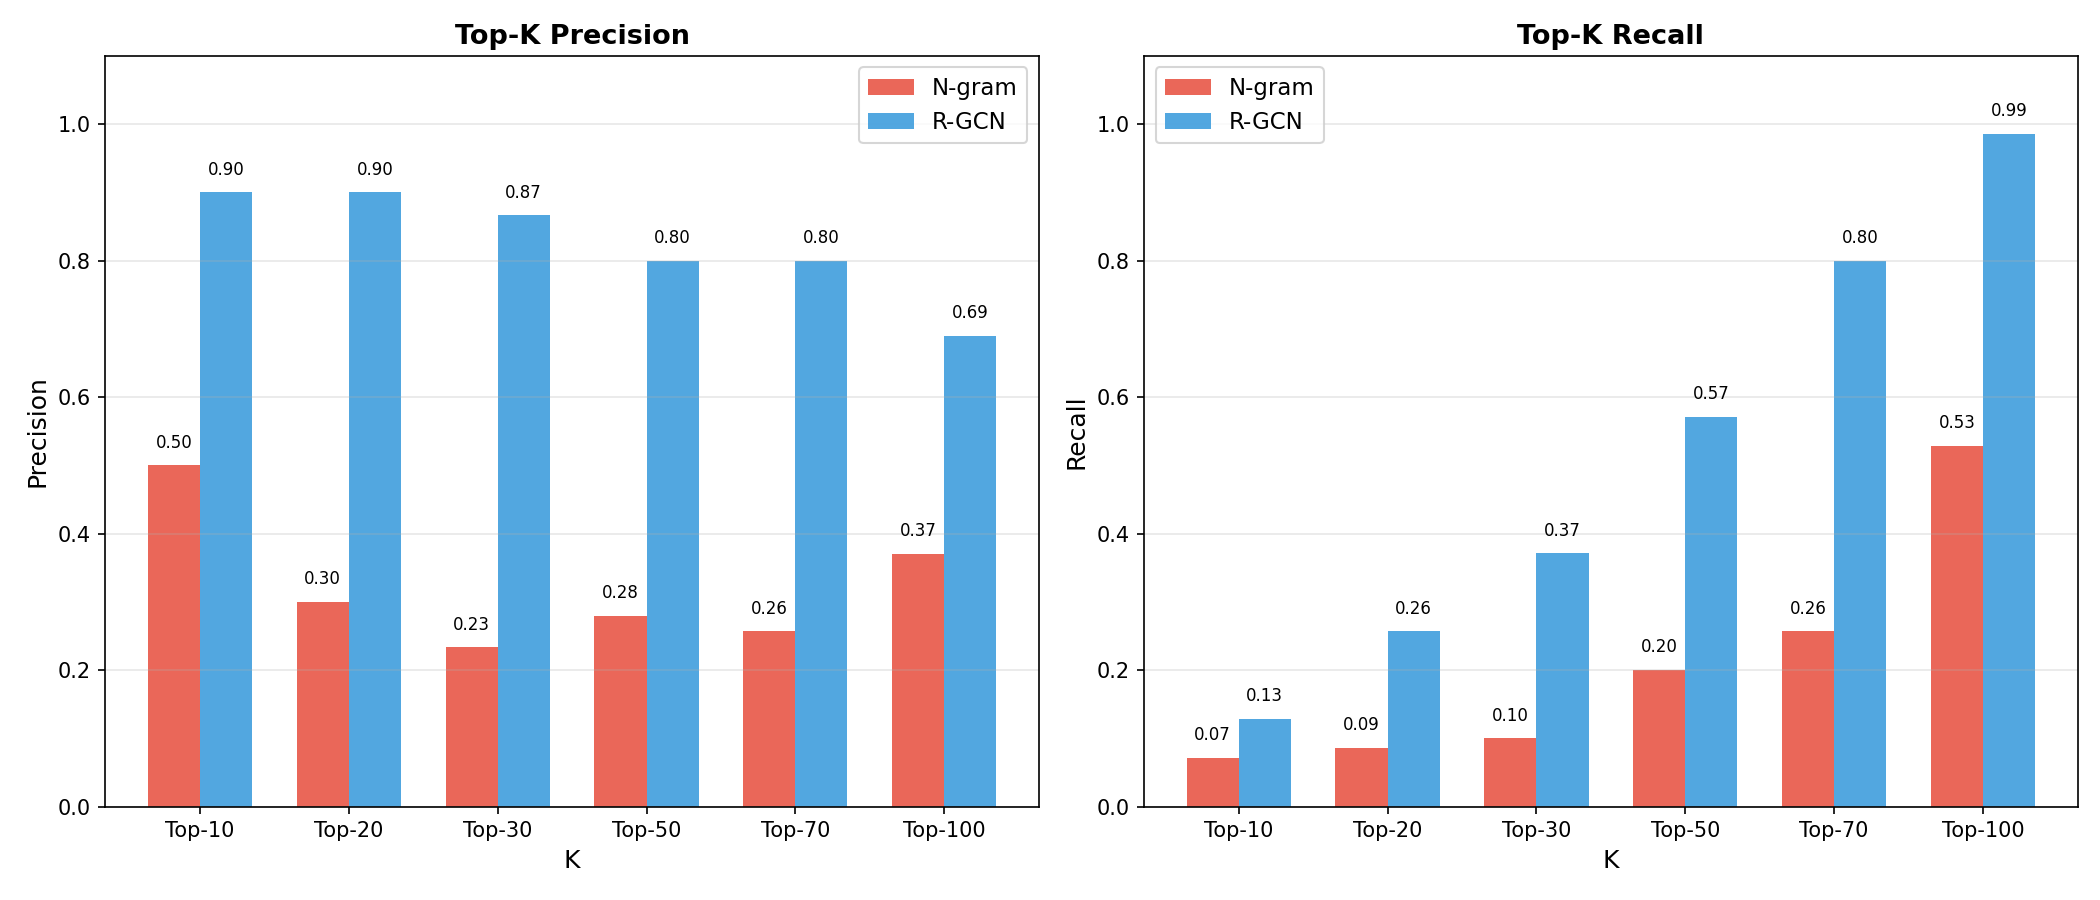
\includegraphics[keepaspectratio,alt={Top-K Precision and Recall Comparison}]{outputs/comparison/fig_topk_comparison.png}}

Figure 3 compares Top-K precision and recall. R-GCN outperforms N-gram
at every K from Top-10 to Top-100, reaching 80\% recall by Top-70, which
is especially useful when analysts can only review a limited number of
users.

\subsubsection{7.3 Scenario-Level Detection
Comparison}\label{73-scenario-level-detection-comparison}

{\def\LTcaptype{none} % do not increment counter
\begin{longtable}[]{@{}llrrrrr@{}}
\toprule\noalign{}
Scenario & Description & Users & N-gram Top-70 & R-GCN Top-70 & N-gram
Top-100 & R-GCN Top-100 \\
\midrule\noalign{}
\endhead
\bottomrule\noalign{}
\endlastfoot
S1 & USB + Leak Upload & 30 & 0.3667 & \textbf{0.7667} & 0.8333 &
\textbf{1.0000} \\
S2 & Job-Hunt + Email Exfil & 30 & 0.0667 & \textbf{0.8667} & 0.1667 &
\textbf{0.9667} \\
S3 & Keylogger & 10 & 0.5000 & \textbf{0.7000} & 0.7000 &
\textbf{1.0000} \\
\end{longtable}
}

\textbf{The S2 scenario shows the most striking difference}: N-gram
detects only 16.67\% of S2 malicious users in the Top-100 (5/30), while
R-GCN detects 96.67\% (29/30). This is because S2 behavioral features
(job-site browsing + document emailing) heavily overlap with benign
users --- 83\% of benign users also have job-hunting site visit records.
The N-gram approach sets the weight of \texttt{HTTP\_JOBHUNT\_WH} to 0
(treating it as noise), causing S2 detection to rely almost entirely on
weak signals. In contrast, R-GCN automatically learns finer-grained
discriminative features from user-PC-URL interaction patterns in the
graph structure.

S1 and S3 scenarios both achieve 100\% recall within
R-GCN\textquotesingle s Top-100.

\pandocbounded{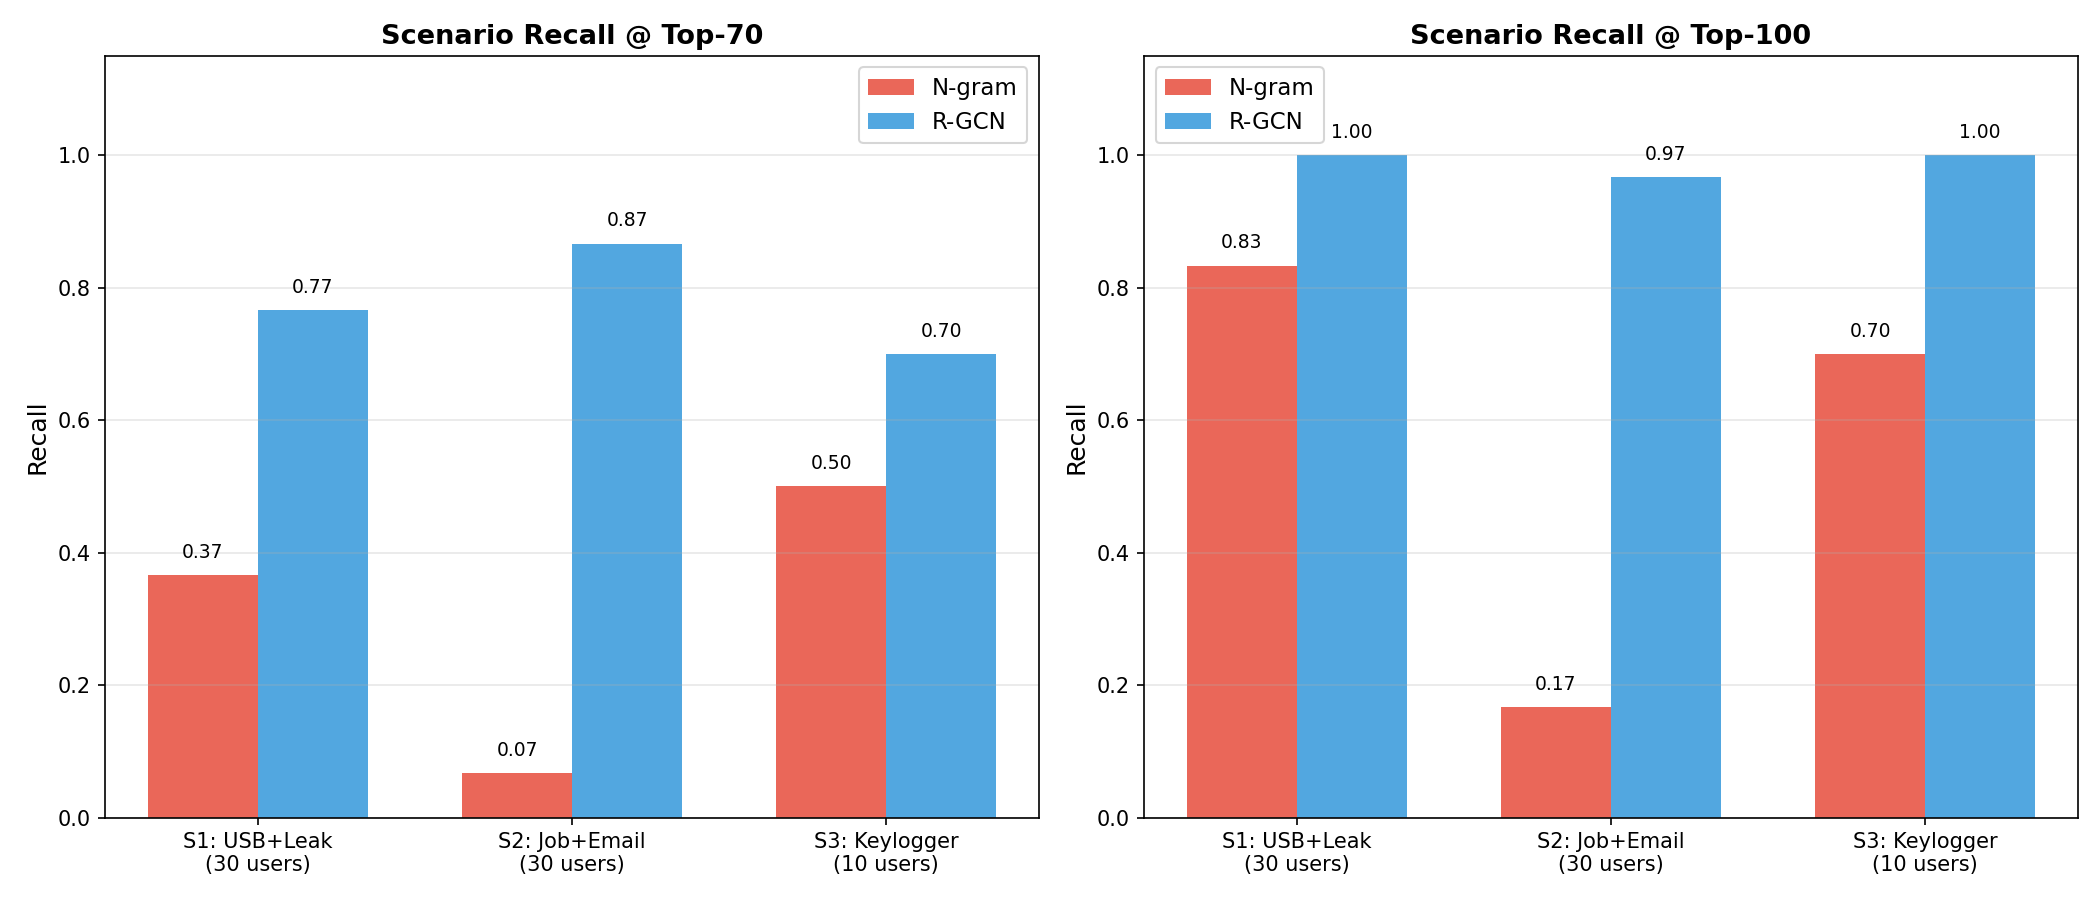
\includegraphics[keepaspectratio,alt={Scenario-Level Recall Comparison}]{outputs/comparison/fig_scenario_comparison.png}}

Figure 4 compares scenario-level Top-70 and Top-100 recall. The S2
improvement is the most pronounced, showing that heterogeneous graph
structure can compensate for weak token-level signals.

\subsubsection{7.4 N-gram Approach Detailed
Results}\label{74-n-gram-approach-detailed-results}

\paragraph{7.4.1 Evaluation Set vs. Full Dataset
Comparison}\label{741-evaluation-set-vs-full-dataset-comparison}

{\def\LTcaptype{none} % do not increment counter
\begin{longtable}[]{@{}lrr@{}}
\toprule\noalign{}
Metric & Full 1,000 Users & Held-Out Evaluation Set (349 Users) \\
\midrule\noalign{}
\endhead
\bottomrule\noalign{}
\endlastfoot
Malicious Users & 70 & 70 \\
Benign Users & 930 & 279 \\
ROC-AUC & 0.9041 & 0.9053 \\
PR-AUC & 0.3257 & 0.6076 \\
Top-50 Precision & 0.2800 & 0.6600 \\
Top-100 Recall & 0.5286 & 0.8143 \\
\end{longtable}
}

PR-AUC is significantly higher on the evaluation set, primarily because
the malicious sample proportion is higher (70/349 = 20\%) compared to
the full dataset (7\%).

\pandocbounded{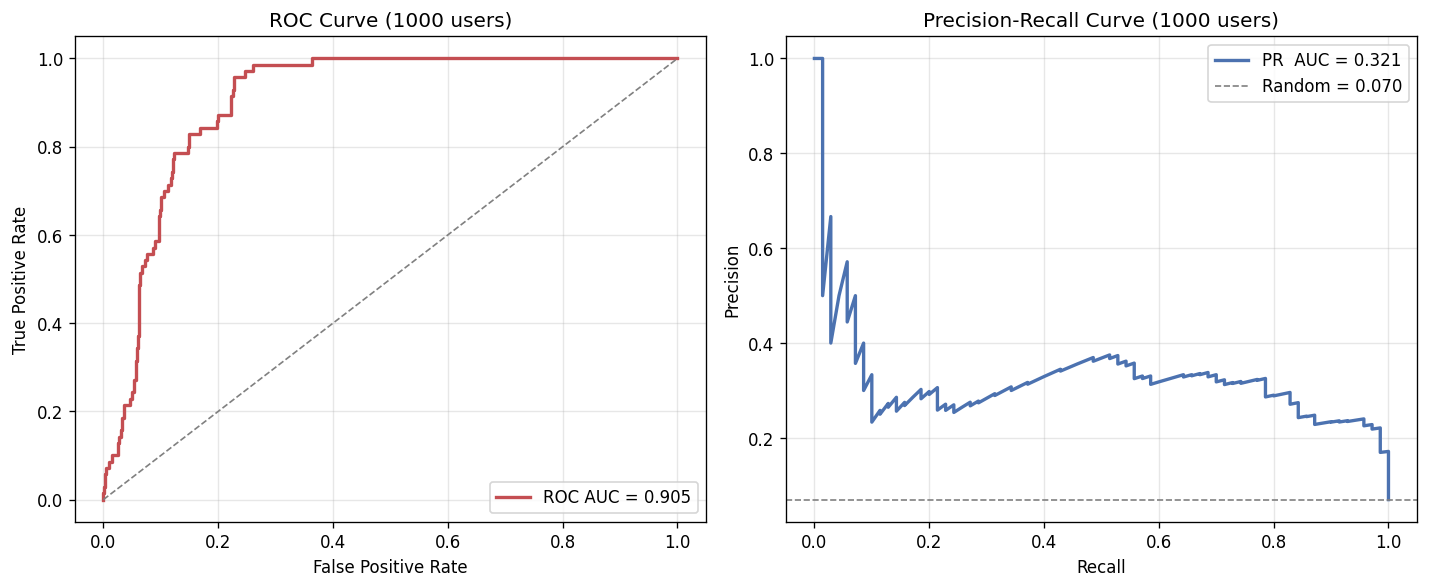
\includegraphics[keepaspectratio,alt={N-gram ROC and PR Curves}]{outputs/fig_roc_pr.png}}

Figure 5 shows the N-gram approach\textquotesingle s standalone ROC and
PR curves. The method has reasonable overall ranking ability, but its PR
curve drops quickly in high-recall regions under sparse positive
samples.

\pandocbounded{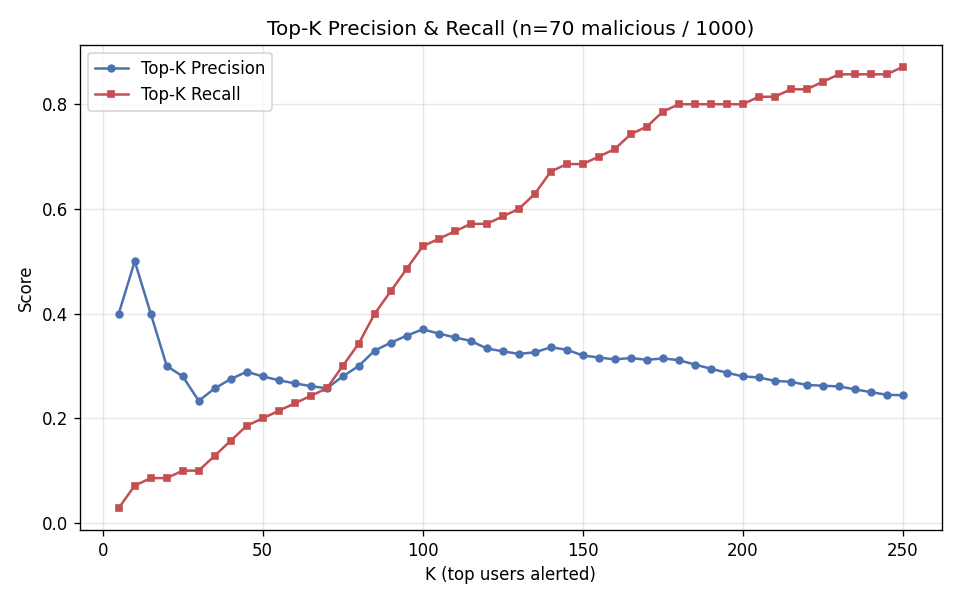
\includegraphics[keepaspectratio,alt={N-gram Top-K Precision and Recall}]{outputs/fig_topk.png}}

Figure 6 shows the N-gram approach\textquotesingle s Top-K trend. Recall
increases as K grows, but precision fluctuates noticeably, reflecting
false positives among benign but highly active users.

\paragraph{7.4.2 Risk Score
Distribution}\label{742-risk-score-distribution}

Among all users, benign users have a mean risk score of 0.1176 (median
0.0870), while malicious users have a mean of 0.3304 (median 0.3250).
The two distributions show some separation, but with considerable
overlap --- the highest benign score reaches 0.7927, contributing to
lower precision.

\pandocbounded{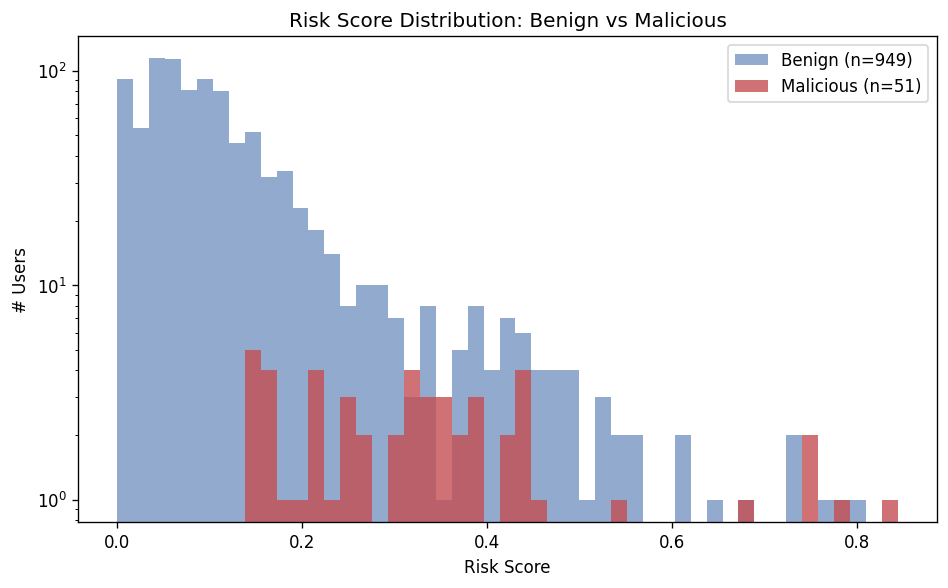
\includegraphics[keepaspectratio,alt={N-gram Risk Score Distribution}]{outputs/fig_risk_distribution.png}}

Figure 7 shows the N-gram risk score distribution. Malicious users shift
to the right overall, but benign and malicious distributions still
overlap substantially, limiting Top-K precision.

\paragraph{7.4.3 Detector Contribution
Analysis}\label{743-detector-contribution-analysis}

Among the N-gram approach\textquotesingle s Top-20 highest-risk users, 5
are true malicious users:

\begin{itemize}
\tightlist
\item
  CCA0046 (S3, rank 1): PatternRule, SequenceSimilarity, and
  PeerDeviation all significantly elevated;
\item
  MPM0220 (S3, rank 3): strong keylogger signature match;
\item
  BSS0369 (S3, rank 6): highest similarity with the S3 signature
  sequence.
\end{itemize}

S3 scenario users consistently rank high because keylogger-related
tokens are rare and carry high threat weights (8.0). S2 scenario users
are the most dispersed, with the worst rank reaching position 408.

\pandocbounded{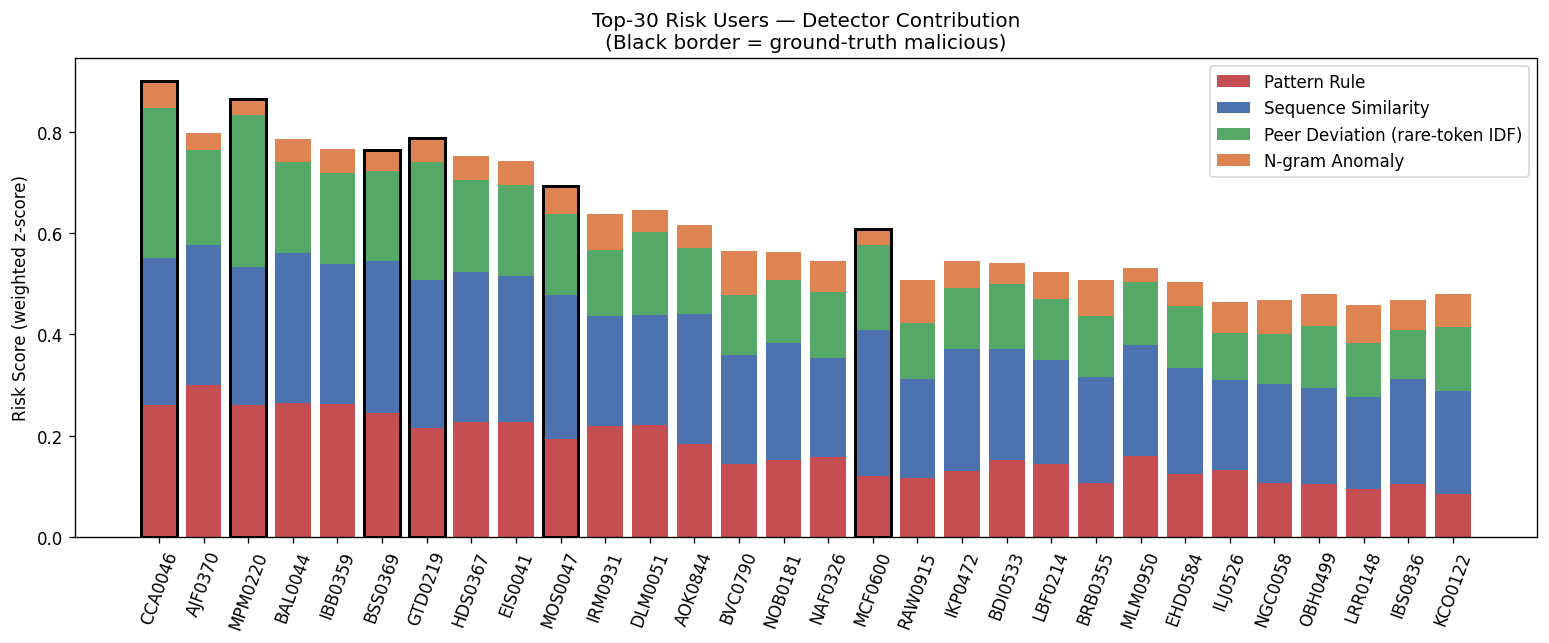
\includegraphics[keepaspectratio,alt={N-gram Top-30 Detector Contribution}]{outputs/fig_top30_contribution.png}}

Figure 8 shows the contribution of the four N-gram detectors among the
Top-30 high-risk users. Black borders mark true malicious users,
illustrating how some malicious users are elevated by multiple detectors
while some benign users receive high scores due to rule or rare-token
matches.

\pandocbounded{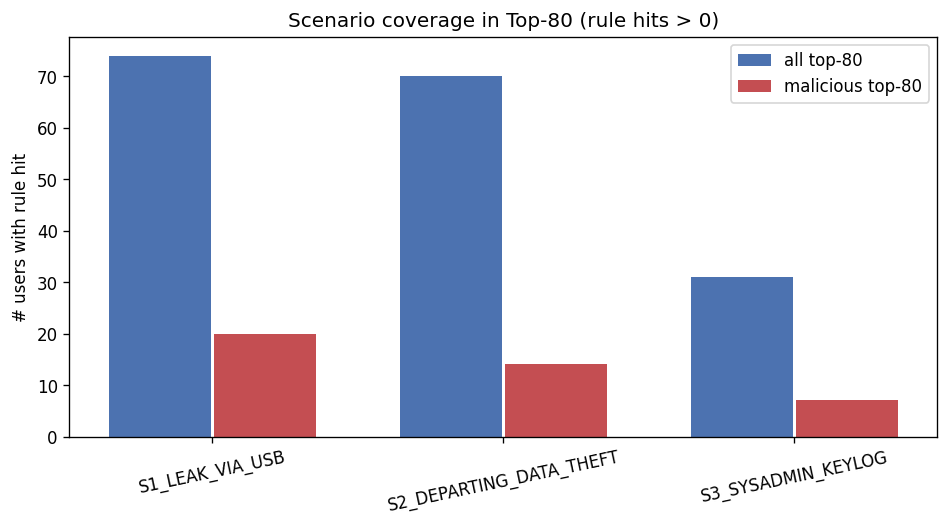
\includegraphics[keepaspectratio,alt={N-gram Scenario Coverage}]{outputs/fig_scenario_breakdown.png}}

Figure 9 shows N-gram scenario coverage within the Top-80 users. S1 and
S3 rule hits are more concentrated, while S2 coverage remains weak,
consistent with the scenario-level recall results.

\pandocbounded{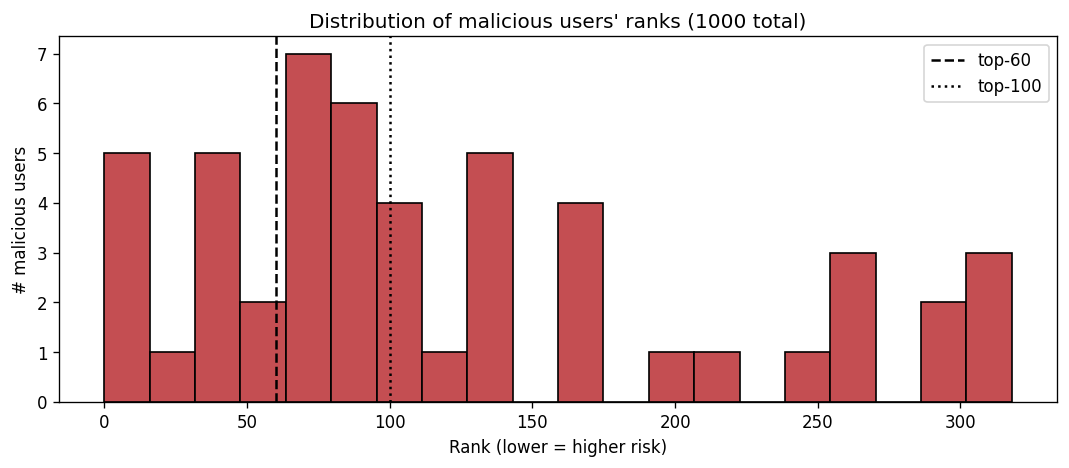
\includegraphics[keepaspectratio,alt={N-gram Malicious User Rank Distribution}]{outputs/fig_malicious_ranks.png}}

Figure 10 shows the rank distribution of all 70 malicious users under
the N-gram full-user ranking. Earlier ranks are more useful for manual
investigation; S2 users tend to appear later and remain the main
optimization target.

\subsubsection{7.5 R-GCN Approach Detailed
Results}\label{75-r-gcn-approach-detailed-results}

\paragraph{7.5.1 Cross-Validation
Stability}\label{751-cross-validation-stability}

{\def\LTcaptype{none} % do not increment counter
\begin{longtable}[]{@{}rllrr@{}}
\toprule\noalign{}
Fold & Training Set & Validation Set & Val AUC & Best Epoch \\
\midrule\noalign{}
\endhead
\bottomrule\noalign{}
\endlastfoot
1 & 800 (56 mal / 744 ben) & 200 (14 mal / 186 ben) & 0.9981 & 36 \\
2 & 800 (56 mal / 744 ben) & 200 (14 mal / 186 ben) & 0.9923 & 32 \\
3 & 800 (56 mal / 744 ben) & 200 (14 mal / 186 ben) & 0.9939 & 22 \\
4 & 800 (56 mal / 744 ben) & 200 (14 mal / 186 ben) & 0.9866 & 29 \\
5 & 800 (56 mal / 744 ben) & 200 (14 mal / 186 ben) & 0.9885 & 37 \\
\textbf{Mean ± Std} & & & \textbf{0.9919 ± 0.0041} & \\
\end{longtable}
}

All fold AUCs exceed 0.98 with a standard deviation of only 0.004,
demonstrating stable performance across different data splits. Early
stopping epochs concentrate in the 22--37 range, indicating rapid
convergence.

\paragraph{7.5.2 OOF Ranking Analysis}\label{752-oof-ranking-analysis}

All of R-GCN\textquotesingle s Top-10 users are malicious (100\%
precision), and only 4 benign users appear among the top 30. The
highest-scoring malicious user (JRG0207) achieves a predicted
probability of 0.9995.

Within the Top-100, R-GCN identifies 69/70 malicious users; the single
missed user ranks only slightly beyond 100, approaching near-perfect
recall.

\pandocbounded{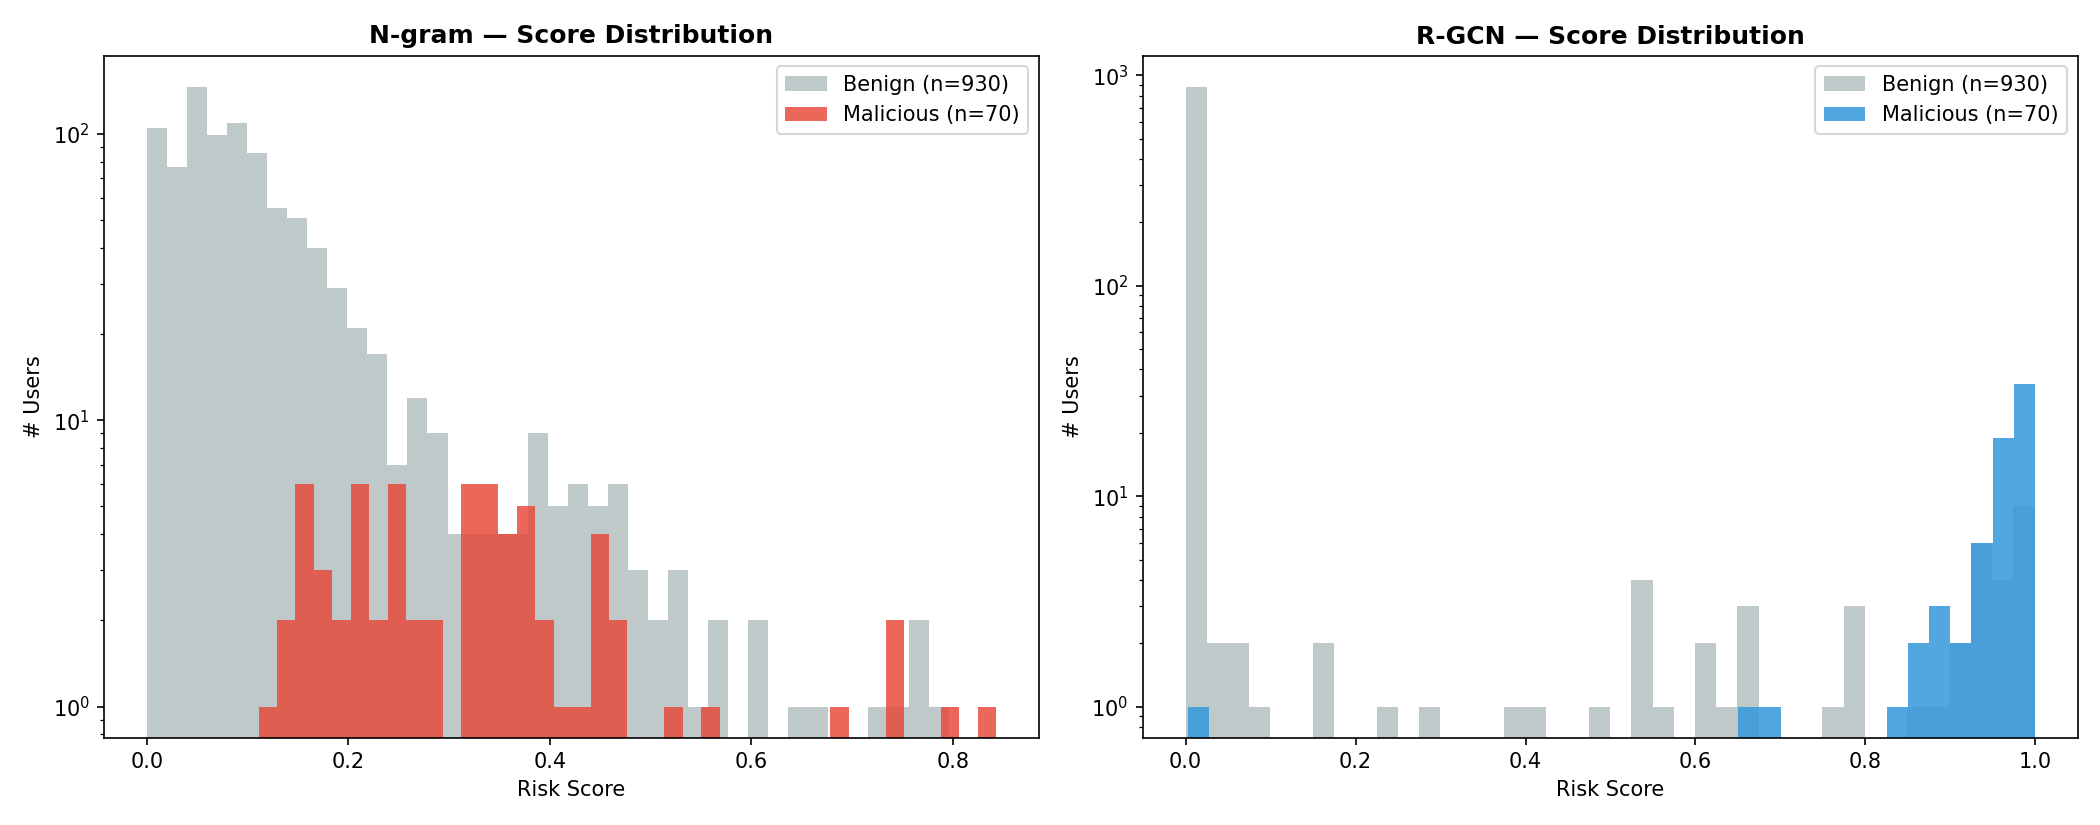
\includegraphics[keepaspectratio,alt={Dual-Algorithm Risk Score Distribution Comparison}]{outputs/comparison/fig_score_dist_comparison.png}}

Figure 11 compares the risk score distributions of the two approaches.
R-GCN separates benign and malicious users more clearly, with malicious
users concentrated in the high-score region; N-gram shows more overlap,
leading to more benign users mixed into the high-risk list.

\subsection{8. Performance Difference
Analysis}\label{8-performance-difference-analysis}

\subsubsection{8.1 Sources of R-GCN\textquotesingle s
Advantage}\label{81-sources-of-r-gcns-advantage}

\begin{enumerate}
\def\labelenumi{\arabic{enumi}.}
\item
  \textbf{Graph Structural Information}: R-GCN leverages relationships
  among users, PCs, files, and URLs through message passing. For
  example, if multiple malicious users share certain PCs or access the
  same sensitive URL categories, these structural patterns propagate
  through graph convolutions, enhancing classification of neighboring
  nodes.
\item
  \textbf{Automatic Feature Learning}: Without manual definition of
  behavioral templates or threat weights, R-GCN automatically learns
  discriminative feature combinations from labeled training data. This
  enables the model to capture complex interaction patterns that human
  experts would find difficult to predefine.
\item
  \textbf{S2 Scenario Breakthrough}: Job-hunting + email exfiltration
  behaviors are individually unremarkable, but their correlation
  patterns with other malicious indicators in the graph structure (e.g.,
  interaction patterns with specific PC clusters or file types) can be
  automatically learned. The N-gram approach sets
  \texttt{HTTP\_JOBHUNT\_WH} weight to 0, effectively discarding this
  dimension entirely.
\item
  \textbf{Semi-supervised Learning Paradigm}: R-GCN fully leverages the
  70 known malicious labels for supervised training, whereas the N-gram
  approach is essentially unsupervised (fitting baselines only on benign
  users), underutilizing known malicious patterns.
\end{enumerate}

\subsubsection{8.2 Unique Advantages of the N-gram
Approach}\label{82-unique-advantages-of-the-n-gram-approach}

Despite R-GCN\textquotesingle s comprehensive numerical superiority, the
N-gram approach retains irreplaceable value:

\begin{enumerate}
\def\labelenumi{\arabic{enumi}.}
\item
  \textbf{Interpretability}: Each high-risk user can be traced to
  specific rule templates ("matched S1\_LEAK\_VIA\_USB template 3
  times"), specific behaviors ("HTTP\_LEAK\_AH events occurred 12
  times"), and specific detectors ("PeerDeviation anomaly"). This is
  critical for SOC operations and internal audits.
\item
  \textbf{No Label Requirement}: In real-world environments, malicious
  user labels are extremely scarce or nonexistent. The N-gram approach
  only requires a benign behavior baseline to operate, making it
  suitable for cold-start scenarios.
\item
  \textbf{Domain Knowledge Integration}: Security expert experience can
  be directly encoded as behavioral templates and threat weights, giving
  the model immediate response capability to known attack patterns.
\item
  \textbf{Computational Efficiency}: The N-gram approach requires no
  GPU, no iterative optimization during training, and is easier to
  deploy in resource-constrained environments.
\end{enumerate}

\subsubsection{8.3 Complementarity of the Two
Approaches}\label{83-complementarity-of-the-two-approaches}

{\def\LTcaptype{none} % do not increment counter
\begin{longtable}[]{@{}lll@{}}
\toprule\noalign{}
Dimension & N-gram & R-GCN \\
\midrule\noalign{}
\endhead
\bottomrule\noalign{}
\endlastfoot
Detection Capability & Moderate (AUC 0.90) & Excellent (AUC 0.99) \\
Interpretability & Strong (rule + template tracing) & Weak (black-box
embeddings) \\
Label Dependency & None (unsupervised) & Required (needs malicious
labels) \\
S2 Scenario & Poor (Recall 17\%) & Excellent (Recall 97\%) \\
Cold Start & Feasible & Requires initial labels \\
Computational Cost & Low & Moderate \\
\end{longtable}
}

\subsection{9. Interpretability
Analysis}\label{9-interpretability-analysis}

The N-gram approach\textquotesingle s primary advantage lies in its
interpretability structure:

\begin{itemize}
\tightlist
\item
  \textbf{PatternRule} answers "Which red-team behavioral templates did
  the user match?";
\item
  \textbf{SequenceSimilarity} answers "Which type of malicious signature
  does the user\textquotesingle s overall sequence most resemble?";
\item
  \textbf{PeerDeviation} answers "What high-risk behaviors does the user
  exhibit that are rare among peers?";
\item
  \textbf{NGramAnomaly} answers "Is the user\textquotesingle s behavior
  abnormal under the benign language model?".
\end{itemize}

This explanation structure is well-suited for SOC or internal audit
scenarios. Analysts can first review the Top-K rankings, then use the
scenario match details in \texttt{outputs/top\_risk\_explanations.json}
to locate specific behavioral chains, rather than receiving only an
opaque classification probability.

The R-GCN approach has weaker interpretability, but can be partially
compensated through post-hoc explanation techniques such as node
embedding analysis, relational attention weights, or gradient
attribution.

\subsection{10. Limitations}\label{10-limitations}

\subsubsection{10.1 Data Level}\label{101-data-level}

\begin{itemize}
\tightlist
\item
  Ground truth relies on the official red-team roster and does not cover
  unknown attack types in real business environments;
\item
  Behavioral token granularity is relatively coarse; file paths, email
  body text, recipient relationships, and role-based access permissions
  are not fully utilized;
\item
  R-GCN currently does not use email.csv data (1.3 GB), potentially
  missing critical email behavior features for S2 and S3 scenarios.
\end{itemize}

\subsubsection{10.2 Method Level}\label{102-method-level}

\begin{itemize}
\tightlist
\item
  The N-gram approach\textquotesingle s fusion weights are manually
  specified and have not been systematically tuned through
  cross-validation or Bayesian optimization;
\item
  The N-gram language model uses only a population-level benign baseline
  and has not established individual user historical baselines;
\item
  The R-GCN approach is transductive and cannot directly classify
  previously unseen new users;
\item
  R-GCN currently does not incorporate temporal information --- all
  events are aggregated into static counts, potentially losing temporal
  attack chain patterns.
\end{itemize}

\subsubsection{10.3 Evaluation Level}\label{103-evaluation-level}

\begin{itemize}
\tightlist
\item
  The two approaches use slightly different evaluation protocols: N-gram
  uses 70/30 benign user split + full scoring, while R-GCN uses 5-fold
  CV + OOF aggregation. Although both ultimately report metrics on all
  1,000 users, training information utilization differs;
\item
  R-GCN uses malicious labels for supervised training, while N-gram is
  essentially unsupervised, creating a certain asymmetry in direct
  comparison.
\end{itemize}

\subsection{11. Future Directions}\label{11-future-directions}

\begin{enumerate}
\def\labelenumi{\arabic{enumi}.}
\tightlist
\item
  \textbf{Fuse the advantages of both approaches}: Build an ensemble
  system using N-gram for interpretable initial screening and rule-based
  alerting, and R-GCN for high-accuracy ranking and priority adjustment;
\item
  \textbf{Introduce temporal graphs}: Extend R-GCN to temporal
  heterogeneous graphs (e.g., T-GCN or dynamic graph networks) to
  capture temporal evolution of behavioral sequences;
\item
  \textbf{Incorporate email data}: Add email\_addr nodes and
  send/receive relations to the R-GCN graph to supplement email
  behavioral signals for S2 and S3 scenarios;
\item
  \textbf{Strengthen S2 scenario modeling}: Combine email recipient
  graphs, attachment sizes, file topics, departure time windows, and
  role change information;
\item
  \textbf{Automatic template mining}: Use PrefixSpan, GSP, or SPADE to
  automatically mine discriminative frequent sequences from malicious
  and benign subsets, replacing manual templates;
\item
  \textbf{Learn fusion weights}: Under the constraint of maintaining
  interpretability, use logistic regression or learning-to-rank to
  automatically learn the N-gram four-component weights;
\item
  \textbf{Enhance graph interpretability}: Add GNNExplainer or attention
  mechanisms to R-GCN to output the most influential subgraphs and
  relations for each prediction;
\item
  \textbf{Personalized baselines}: Use each user\textquotesingle s own
  past 30--60 days of behavior as a reference to detect behavioral
  drift, reducing false positives for highly active benign users.
\end{enumerate}

\subsection{12. Conclusion}\label{12-conclusion}

This project implements and compares two insider threat detection
approaches on the complete CMU-CERT r4.2 dataset. The experimental
results demonstrate:

\begin{enumerate}
\def\labelenumi{\arabic{enumi}.}
\item
  \textbf{The R-GCN heterogeneous graph approach significantly
  outperforms the N-gram sequence matching approach in detection
  performance}, with ROC-AUC improving from 0.9041 to 0.9898, PR-AUC
  from 0.3257 to 0.8358, and Top-100 Recall from 52.86\% to 98.57\%.
\item
  \textbf{R-GCN achieves a qualitative breakthrough on the
  hardest-to-detect S2 scenario}, with Top-100 Recall improving from
  16.67\% to 96.67\%. Graph structural information enables the model to
  capture behavioral correlation patterns that rule-based methods cannot
  cover.
\item
  \textbf{The N-gram approach retains unique value in interpretability
  and unsupervised settings}, where each high-risk user can be traced to
  specific rule templates and behavioral patterns, making it suitable
  for SOC operations and cold-start scenarios.
\item
  \textbf{The two approaches are complementary}, and future work can
  build an ensemble system combining R-GCN\textquotesingle s high
  accuracy with N-gram\textquotesingle s interpretability.
\end{enumerate}

Overall, this project provides empirical evidence for method selection
in insider threat detection: when labeled data is available, graph
neural network methods offer clear advantages; in label-free or
interpretability-critical scenarios, domain-knowledge-driven sequence
matching remains a viable choice.

\subsection{Appendix A: Project File
Reference}\label{appendix-a-project-file-reference}

{\def\LTcaptype{none} % do not increment counter
\begin{longtable}[]{@{}ll@{}}
\toprule\noalign{}
File & Purpose \\
\midrule\noalign{}
\endhead
\bottomrule\noalign{}
\endlastfoot
\texttt{src/preprocess.py} & Multi-source log streaming, behavioral
tokenization, user sequence construction \\
\texttt{src/build\_ground\_truth.py} & CMU-CERT r4.2 official malicious
user list (70 users) \\
\texttt{src/sequence\_matching.py} & N-gram approach: four detectors and
risk fusion model \\
\texttt{src/train\_evaluate.py} & N-gram approach: training, scoring,
evaluation, and explanation output \\
\texttt{src/visualize.py} & N-gram approach: evaluation chart
generation \\
\texttt{src/rgcn/build\_graph.py} & R-GCN approach: heterogeneous graph
construction \\
\texttt{src/rgcn/rgcn\_model.py} & R-GCN approach: model architecture
definition \\
\texttt{src/rgcn/train\_rgcn.py} & R-GCN approach: training and
evaluation \\
\texttt{src/generate\_http\_slim.py} & Utility: generate slim
http\_slim.csv from http.csv \\
\texttt{src/compare\_algorithms.py} & Dual-algorithm performance
comparison and visualization \\
\texttt{src/run\_full\_pipeline.py} & One-click full pipeline runner \\
\end{longtable}
}

\subsection{Appendix B: Output File
Inventory}\label{appendix-b-output-file-inventory}

{\def\LTcaptype{none} % do not increment counter
\begin{longtable}[]{@{}ll@{}}
\toprule\noalign{}
File & Contents \\
\midrule\noalign{}
\endhead
\bottomrule\noalign{}
\endlastfoot
\texttt{outputs/metrics.json} & N-gram approach evaluation metrics \\
\texttt{outputs/risk\_scores.csv} & N-gram approach full user risk
scores \\
\texttt{outputs/malicious\_user\_ranking.csv} & N-gram approach
malicious user rankings \\
\texttt{outputs/top\_risk\_explanations.json} & N-gram approach Top-80
user explanations \\
\texttt{outputs/fig\_*.png} & N-gram approach visualization charts (6
figures) \\
\texttt{outputs/rgcn/graph.pt} & R-GCN heterogeneous graph data \\
\texttt{outputs/rgcn/rgcn\_results.json} & R-GCN evaluation metrics and
Top-30 ranking \\
\texttt{outputs/rgcn/rgcn\_results.csv} & R-GCN full user risk
ranking \\
\texttt{outputs/comparison/comparison\_report.json} & Dual-algorithm
comparison data \\
\texttt{outputs/comparison/comparison\_report.md} & Dual-algorithm
comparison report \\
\texttt{outputs/comparison/fig\_*.png} & Comparison visualization charts
(5 figures) \\
\end{longtable}
}

\subsection{Appendix C: Figure Index}\label{appendix-c-figure-index}

{\def\LTcaptype{none} % do not increment counter
\begin{longtable}[]{@{}lll@{}}
\toprule\noalign{}
Figure & Description & File \\
\midrule\noalign{}
\endhead
\bottomrule\noalign{}
\endlastfoot
Figure 1 & Dual-algorithm ROC curve comparison &
\texttt{outputs/comparison/fig\_roc\_comparison.png} \\
Figure 2 & Dual-algorithm Precision-Recall curve comparison &
\texttt{outputs/comparison/fig\_pr\_comparison.png} \\
Figure 3 & Dual-algorithm Top-K Precision/Recall comparison &
\texttt{outputs/comparison/fig\_topk\_comparison.png} \\
Figure 4 & Dual-algorithm scenario-level Recall comparison &
\texttt{outputs/comparison/fig\_scenario\_comparison.png} \\
Figure 5 & N-gram ROC and PR curves &
\texttt{outputs/fig\_roc\_pr.png} \\
Figure 6 & N-gram Top-K Precision and Recall &
\texttt{outputs/fig\_topk.png} \\
Figure 7 & N-gram risk score distribution &
\texttt{outputs/fig\_risk\_distribution.png} \\
Figure 8 & N-gram Top-30 detector contribution &
\texttt{outputs/fig\_top30\_contribution.png} \\
Figure 9 & N-gram scenario coverage &
\texttt{outputs/fig\_scenario\_breakdown.png} \\
Figure 10 & N-gram malicious user rank distribution &
\texttt{outputs/fig\_malicious\_ranks.png} \\
Figure 11 & Dual-algorithm risk score distribution comparison &
\texttt{outputs/comparison/fig\_score\_dist\_comparison.png} \\
\end{longtable}
}

\subsection{Appendix D: Environment and
Reproducibility}\label{appendix-d-environment-and-reproducibility}

\begin{Shaded}
\begin{Highlighting}[]
\CommentTok{\# Activate virtual environment}
\BuiltInTok{source}\NormalTok{ \textasciitilde{}/.virtualenvs/demo4{-}env/bin/activate}

\CommentTok{\# One{-}click full pipeline}
\ExtensionTok{python}\NormalTok{ src/run\_full\_pipeline.py}

\CommentTok{\# Or run step by step:}
\ExtensionTok{python}\NormalTok{ src/generate\_http\_slim.py         }\CommentTok{\# Step 0: Generate http\_slim.csv (if not exists)}
\ExtensionTok{python}\NormalTok{ src/preprocess.py                  }\CommentTok{\# Step 1: N{-}gram preprocessing}
\ExtensionTok{python}\NormalTok{ src/train\_evaluate.py              }\CommentTok{\# Step 2: N{-}gram training and evaluation}
\ExtensionTok{python}\NormalTok{ src/visualize.py                   }\CommentTok{\# Step 3: N{-}gram visualization}
\ExtensionTok{python}\NormalTok{ src/rgcn/build\_graph.py            }\CommentTok{\# Step 4: R{-}GCN graph construction}
\ExtensionTok{python}\NormalTok{ src/rgcn/train\_rgcn.py }\AttributeTok{{-}{-}verbose}   \CommentTok{\# Step 5: R{-}GCN training and evaluation}
\ExtensionTok{python}\NormalTok{ src/compare\_algorithms.py          }\CommentTok{\# Step 6: Dual{-}algorithm comparison}
\end{Highlighting}
\end{Shaded}

\textbf{Dependency Versions}: Python 3.x, pandas 2.1.4, scikit-learn
1.5.0, numpy 1.26.2, PyTorch 2.7.1, matplotlib, tqdm

\end{document}
